\section{AHTR Plank Optimization Results Discussion}
\label{sec:plank-discussion}
In this section, I conduct a deep-dive to understand the driving factors for 
each individual objective, and how their combined effects result in the optimal 
reactor models found by the multi-objective optimization simulations. 

\subsection{Discussion: Minimize $PF_{total}$ Objective}
\label{sec:plank-discussion-pf}
\paragraph{Simulation p-1a}
In Section \ref{sec:plank-1-obj-pf}'s simulation p-1a, I conducted a single-objective 
optimization simulation to minimize total fuel packing fraction ($PF_{total}$) by 
varying $PF_{total}$ and TRISO distribution. 
In simulation p-1a, \gls{ROLLO} found that an \gls{AHTR} plank model with a
$PF_{total}$ = 0.023 and oscillating TRISO distribution most-minimized 
$PF_{total}$ while meeting the $k_{eff} \geq 1.35$ constraint 
(Figure \ref{fig:slab-obj-1-pf}). 

I ran a simulation for constant $PF_{total}$ = 0.023 TRISO distribution and compared its 
fission reaction rate with the oscillating TRISO distribution 
to understand why the oscillating TRISO distribution enabled a lower $PF_{total}$. 
Figure \ref{fig:triso-0.023} shows the TRISO distributions for the two compared 
simulations: Figure \ref{fig:slab-obj-1-pf}'s most-minimized $PF_{total}$ 
and the constant $PF_{total}$ = 0.023. 
\begin{figure}[htbp!]
    \centering
    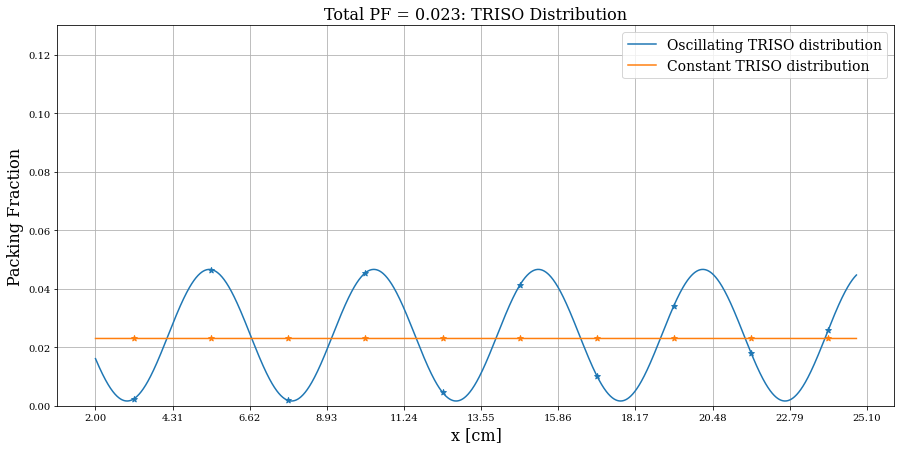
\includegraphics[width=0.9\linewidth]{triso-0.023.png} 
    \caption{Simulation p-1a's most-minimized $PF_{total}$ TRISO distribution 
    (oscillating TRISO distribution) from Figure \ref{fig:slab-obj-1-pf} and the 
    constant $PF_{total}$ = 0.023 TRISO distribution.}
    \label{fig:triso-0.023}
\end{figure}

Table \ref{tab:0.023-plank-fission-rate} compares the total fission reaction rate 
(OpenMC's \texttt{fission} tally) between the most-minimized $PF_{total}$ TRISO 
distribution and a constant $PF_{total}$ = 0.023 TRISO distribution (both shown in 
Figure \ref{fig:triso-0.023}).
\begin{table}[htbp!]
    \centering
    \onehalfspacing
    \caption{Total fission reaction rate comparison between the most-minimized 
    $PF_{total}$ TRISO distribution and a constant $PF_{total}$ = 0.023 TRISO 
    distribution.}
	\label{tab:0.023-plank-fission-rate}
    \footnotesize
    \begin{tabular}{p{2cm}lp{4cm}p{2.7cm}p{4cm}}
    \hline
    \textbf{Energy Group} & 
    \textbf{$\%$ of Total} &
    \textbf{Most-minimized $PF_{total}$ fission [reactions/src]} & 
    \textbf{Flat $PF_{total}$ fission [reactions/src]} & 
    \textbf{$\%$ fission difference}\\
    \hline 
    1 & 0.21 & 0.001260 & 0.001234 & \Plus2.07 \\
    2 & 1.16 & 0.006653 & 0.006658 & \Minus0.07 \\
    3 & 1.15 & 0.006566 & 0.006580 & \Minus0.21 \\
    4 & 97.46 & 0.556897 & 0.555889 & \Plus0.18 \\
    \hline
    \end{tabular}
\end{table}
In energy group 4, the most-minimized $PF_{total}$ TRISO distribution has $0.18\%$ higher  
\texttt{fission} (total fission reaction rate) than the constant 
$PF_{total}$ = 0.023 TRISO distribution, explaining why the oscillating TRISO 
distribution enabled a lower packing fraction for the same $k_{eff}$ compared to the 
constant TRISO distribution. 

\paragraph{Simulation p-1d}
In Section \ref{sec:plank-1-obj-pf}'s simulation p-1d, I conducted a single-objective 
optimization simulation to minimize total fuel packing fraction ($PF_{total}$) by 
varying $PF_{total}$ and coolant channel shape. 
In simulation p-1a, \gls{ROLLO} found that there is no correlation 
between $PF_{total}$ and coolant channel shape (demonstrated in Figure 
\ref{fig:slab-obj-1-pf-final-coolant}). 

\paragraph{Summary}
The minimize $PF_{total}$ objective is driven by maximizing the total fission reaction 
rates in the thermal energy group (Group 4). 
The minimize $PF_{total}$ objective has correlations with the following input parameters: 
$PF_{total}$ and TRISO packing fraction distribution. 
The objective has no correlation with coolant channel shape input parameter. 

\subsection{Discussion: Minimize $T_{max}$ Objective}
\label{sec:plank-discussion-temp}
\paragraph{Simulation p-1b}
In Section \ref{sec:plank-1-obj-temp}'s simulation p-1b, I conducted a single-objective 
optimization simulation to minimize maximum plank temperature ($T_{max}$) by varying 
TRISO distribution. 
In simulation p-1b, \gls{ROLLO} found that an \gls{AHTR} plank model with a mostly 
flat TRISO distribution most-minimized $T_{max}$ 
(Figure \ref{fig:slab-obj-1-temp-final}).

I found that a fully flat \gls{TRISO} distribution results in a higher $T_{max}$.
Figure \ref{fig:slab-obj-1-temp-distr} compares the Moltres-generated centerline 
temperature distribution for the plank with mostly flat (Figure 
\ref{fig:slab-obj-1-temp-final}) and flat TRISO distributions for the same 
$PF_{total}$ = 0.0979. 
\begin{figure}[htbp!]
    \centering
    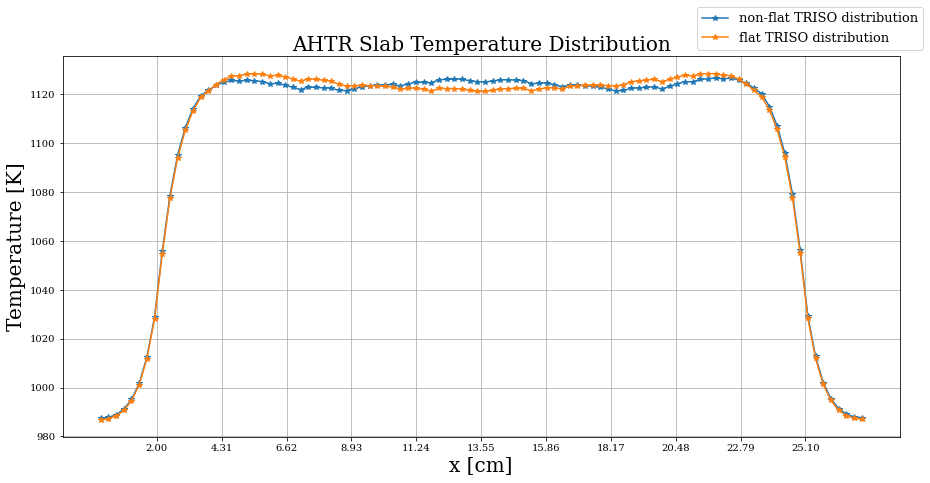
\includegraphics[width=\linewidth]{slab-obj-1-temp-distr.png}
    \caption{Comparison of Moltres-generated AHTR plank temperature distribution for 
    non-flat and flat TRISO distribution. 
    Both models have $PF_{total}$ = 0.0979.}
    \label{fig:slab-obj-1-temp-distr}
\end{figure}
The \gls{AHTR} plank with a flat \gls{TRISO} distribution has higher plank temperatures 
on the left and right sides near the moderator. 
To combat this temperature peak, ROLLO found a \gls{TRISO} distribution that 
has a slight dip near the moderator regions, resulting in a lower $T_{max}$.

\paragraph{Simulation p-1e}
In Section \ref{sec:plank-1-obj-temp}'s simulation p-1e, I conducted a single-objective 
optimization simulation to minimize maximum plank temperature ($T_{max}$) by varying 
coolant channel shape. 
In simulation p-1e, \gls{ROLLO} found that there is a negative linear correlation 
between the plank's $T_{max}$ and total radius ($r_{tot}$), shown in 
Figure \ref{fig:slab-obj-1-temp-final-coolant}. 
Comparison of simulation p-1b and p-1e's results in 
Figures \ref{fig:slab-obj-1-temp-evol} and \ref{fig:slab-obj-1-temp-evol-coolant} 
show that coolant channel shape variation does not have as high of an impact on 
$T_{max}$ as \gls{TRISO} distribution variation: the average $T_{max}$ due to 
\gls{TRISO} variation decreased by 60K over 10 generations, while average $T_{max}$ due 
to coolant channel shape variation only decreased by 15K over 10 generations. 

\paragraph{Summary}
The minimize $T_{max}$ objective is driven by minimizing plank's maximum temperature; 
and flattens TRISO distribution and maximizes coolant channel shape's 
$r_{tot}$ to achieve the objective. 
The minimize $T_{max}$ objective has correlations with all the input parameters: 
$PF_{total}$, TRISO packing fraction distribution, and coolant channel shape. 
The results from simulation p-1b and p-1e suggest that the objective is more heavily 
influenced by the TRISO distribution than the coolant channel shape. 

\subsection{Discussion: Minimize $PPF_{fuel}$ Objective}
\label{sec:plank-discussion-ppf}
In an effort to understand the driving factors for the minimize $PPF_{fuel}$ 
objective, I conduct an equation analysis to determine the \gls{AHTR} plank properties 
that influence $PPF_{fuel}$. 
I then demonstrate the derived relationship in simulation p-1c and p-2b's results. 

\subsubsection{Equation Analysis}
\label{sec:plank-discussion-ppf-equation}
Equation \ref{eq:reaction-rate-fission} shows the relationship between fission reaction 
rate, flux, and material properties: 
\begin{align}
\label{eq:reaction-rate-fission}
    RR_f &= \Phi \times \sigma_f \times N \\
\intertext{where}
    RR_f &= \mbox{fission reaction rate } [reactions \cdot cm^{-3} \cdot s^{-1}] \nonumber \\
    \Phi &= \mbox{neutron flux } [neutrons \cdot cm^{-2} \cdot s^{-1}] \nonumber \\
    \sigma_f &= \mbox{microscopic cross section } [cm^2] \nonumber \\
    N &= \mbox{atomic number density } [atoms \cdot cm^{-3}] \nonumber 
\end{align}

Since microscopic cross section is constant for the same fuel material, I rearrange 
Equation \ref{eq:reaction-rate-fission} into Equation \ref{eq:reaction-rate-fission-prop}: 
\begin{align}
    \label{eq:reaction-rate-fission-prop}
    \Phi \propto \frac{RR_f}{N}
\end{align}
In Section \ref{sec:ahtr_slab_output}, I defined the fuel-normalized power peaking 
factor ($PPF_{fuel}$) as: 
\begin{align}
    PPF_{fuel} &= max(\frac{fqr_j}{PF_j}) \div ave(\frac{fqr_j}{PF_j})
\intertext{where}
PPF_{fuel} &= \mbox{fuel-normalized power peaking factor} \nonumber \\
j &= \mbox{discretized fuel area j} \nonumber \\
fqr_j &= \mbox{fission-q-recoverable at position j (OpenMC tally)} \nonumber \\
PF_j &= \mbox{fuel packing fraction at position j} \nonumber
\end{align}
The fission reaction rate ($RR_f$) is proportional to fission energy production rate 
($fqr$). 
The atomic number density (N) is proportional to the fuel packing fraction ($PF$). 
Thus, I can further rearrange Equation \ref{eq:reaction-rate-fission-prop} into 
Equation \ref{eq:flux-prop-fqr}:
\begin{align}
    \label{eq:flux-prop-fqr}
    \Phi_j \propto \frac{fqr_j}{PF_j}
\end{align}
Finally, I can further rearrange into Equation \ref{eq:flux-prop-ppf}:
\begin{align}
    \label{eq:flux-prop-ppf}
    max(\Phi_j) \div ave(\Phi_j) &\propto max(\frac{fqr_j}{PF_j}) \div ave(\frac{fqr_j}{PF_j}) \nonumber \\
    &\propto PPF_{fuel}
\end{align}

Therefore, from Equation \ref{eq:flux-prop-ppf}, a flatter flux (smaller 
$max(\Phi_j) \div ave(\Phi_j)$ value) will result in a smaller $PPF_{fuel}$. 
Specifically, flatter energy group 4 thermal flux results in a smaller $PPF_{fuel}$
(see Table \ref{tab:fission-flux}). 
Table \ref{tab:fission-flux} shows the percentage contributions of fission reactions from 
each energy group. 
\begin{table}[htbp!]
    \centering
    \onehalfspacing
    \caption{Percentage of fission reactions from each energy group for \gls{AHTR} plank model.}
	\label{tab:fission-flux}
    \footnotesize
    \begin{tabular}{llp{4cm}}
    \hline 
    \textbf{Energy Group} & \textbf{Energy Bounds [MeV]} & \textbf{Percentage of Total Fission Reactions [\%]} \\
    \hline
    1 & $9.1188\times 10^{-3} < E < 2.0000\times 10^1$ & 0.85 \\ 
    2 & $2.9023\times 10^{-5} < E < 9.1188\times 10^{-3}$ & 4.85 \\
    3 & $1.8554\times 10^{-6} < E < 2.9023\times 10^{-5}$ & 4.14 \\
    4 & $1.0000\times 10^{-12} < E < 1.8554\times 10^{-6}$ & 90.14 \\
    \hline
    \end{tabular}
\end{table}
Most fission reactions are occurring in energy group 4. 

In the following section, I demonstrate Equation \ref{eq:flux-prop-ppf}'s relationship 
in simulation p-1c and p-2b's results. 

\subsubsection{Results Analysis}
\label{sec:plank-discussion-ppf-results}

\paragraph{Simulation p-1c}
In Section \ref{sec:plank-1-obj-ppf}'s simulation p-1c, I conducted a single-objective 
optimization simulation to minimize fuel-normalized power peaking factor ($PPF_{fuel}$) 
by varying TRISO distribution. 
In simulation p-1c, \gls{ROLLO} found that for $PF_{total}$ = 0.0979, an \gls{AHTR} 
plank model with TRISO distribution that peaks near the edges of the fuel region of 
the plank and a minimum point in center of the plank with a variation of $\sim0.07$, 
most-minimized $PPF_{fuel}$. 

I ran a simulation for constant $PF_{total}$ = 0.0979 and compared its 
flux to simulation p-1c's most-minimized $PPF_{fuel}$ TRISO distribution to understand 
why the latter enabled a lower $PPF_{fuel}$. 
Figure \ref{fig:triso-0.0979} shows the TRISO distributions with their $PPF_{fuel}$ 
values for the two compared simulations: Figure \ref{fig:slab-obj-1-ppf}'s 
most-minimized $PPF_{fuel}$ TRISO distribution and the constant $PF_{total}$ = 0.0979 
TRISO distribution. 
\begin{figure}[htbp!]
    \centering
    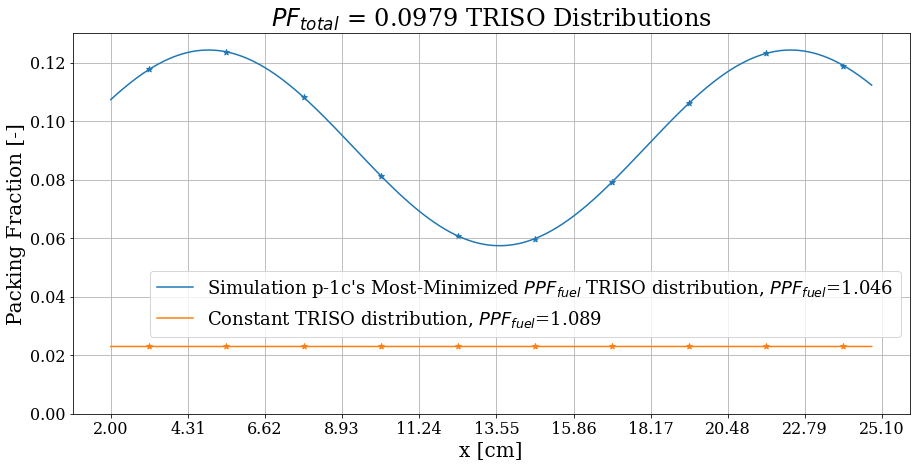
\includegraphics[width=0.9\linewidth]{triso-0.0979.png} 
    \caption{Simulation p-1c's most-minimized $PPF_{fuel}$ TRISO distribution 
    from Figure \ref{fig:slab-obj-1-ppf} and the constant $PF_{total}$ = 0.0979 
    TRISO distribution.}
    \label{fig:triso-0.0979}
\end{figure}

Figure \ref{fig:flux-comparison-0.0979-plank} compares the flux distributions between 
the most-minimized $PPF_{fuel}$ TRISO distribution and the constant $PF_{total}$ = 0.0979 
TRISO distribution (both shown in Figure \ref{fig:triso-0.0979}).
\begin{figure}[htbp!]
    \centering
    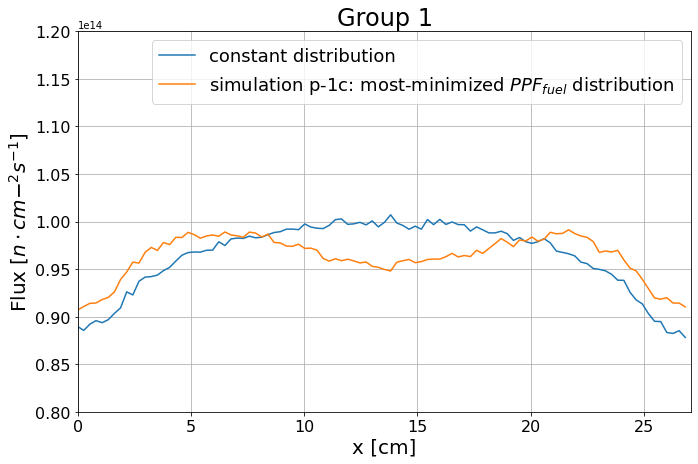
\includegraphics[width=0.48\linewidth]{flux-comparison-0.0979-plank_grp1.png} 
    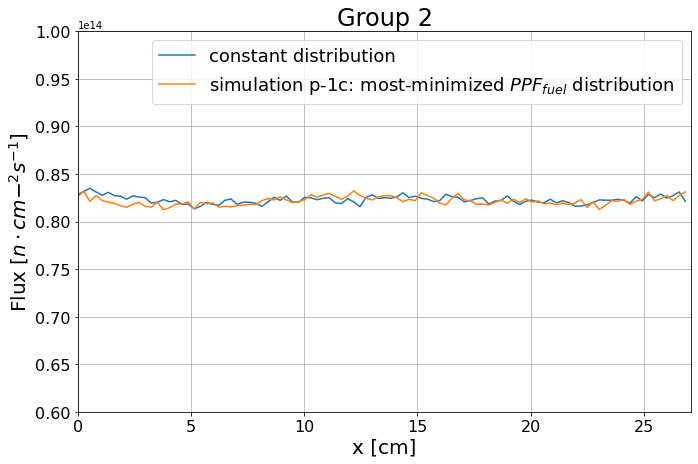
\includegraphics[width=0.48\linewidth]{flux-comparison-0.0979-plank_grp2.png} 
    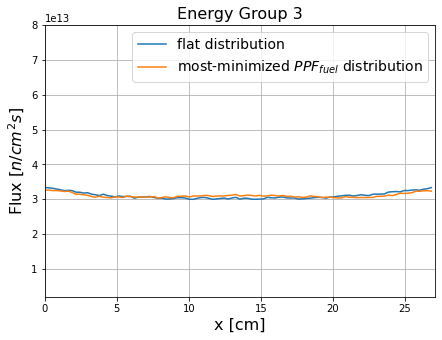
\includegraphics[width=0.48\linewidth]{flux-comparison-0.0979-plank_grp3.png} 
    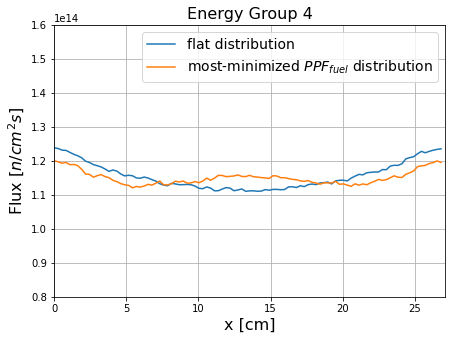
\includegraphics[width=0.48\linewidth]{flux-comparison-0.0979-plank_grp4.png} 
    \caption{Flux comparison between Figure \ref{fig:slab-obj-1-ppf-final}'s TRISO 
    distribution that most-minimized $PPF_{fuel}$ and a constant $PF_{total}$ = 0.0979 
    TRISO distribution. 
    \acrfull{AHTR} plank's centerline neutron flux distribution in 4 groups at 948K. 
    Centerline is the white line in Figure \ref{fig:ahtr-plank-verification}.
    Energy Group 1: E $> 9.1188 \times 10^{-3}$ MeV, 
    Energy Group 2: $2.9023 \times 10^{-5} < E < 9.1188 \times 10^{-3}$ MeV,
    Energy Group 3:  $1.8556 \times 10^{-5} < E < 2.9023 \times 10^{-5}$ MeV,
    Energy Group 4:  $1.0 \times 10^{-12} < E < 1.8554 \times 10^{-6}$ MeV.}
    \label{fig:flux-comparison-0.0979-plank}
\end{figure}

In Figure \ref{fig:flux-comparison-0.0979-plank}, the constant TRISO distribution's 
Group 4 flux dips in the center of the plank due to spatial self-shielding effects. 
In the constant TRISO distribution's Group 1 flux, there is a peak in fast neutrons
born in the plank's center, they are moderated in the graphite matrix and graphite 
structure (Figure \ref{fig:straightened_plank}). 
The self-shielding neutrons are more likely absorbed at the plank's sides, near 
the pure graphite structure moderating regions. 
The outer sides of the plank geometrically shield the plank's center from neutron 
flux, leading to a relatively lower group 4 thermal flux in the plank's center for 
the constant TRISO distribution. 

Table \ref{tab:flux-comparison-0.0979-plank} quantifies the flux comparison 
from Figure \ref{fig:flux-comparison-0.0979-plank} between simulation p-1c's 
most-minimized $PPF_{fuel}$ TRISO distribution and the constant 
$PF_{total}$ = 0.0979 TRISO distribution (both shown in Figure \ref{fig:triso-0.0979}).
\begin{table}[htbp!]
    \centering
    \onehalfspacing
    \caption{Flux value comparison between Figure \ref{fig:slab-obj-1-ppf-final}'s TRISO 
    distribution that most-minimized $PPF_{fuel}$ and a constant $PF_{total}$ = 0.0979 
    TRISO distribution. 
    Energy Group 1: E $> 9.1188 \times 10^{-3}$ MeV, 
    Energy Group 2: $2.9023 \times 10^{-5} < E < 9.1188 \times 10^{-3}$ MeV,
    Energy Group 3:  $1.8556 \times 10^{-5} < E < 2.9023 \times 10^{-5}$ MeV,
    Energy Group 4:  $1.0 \times 10^{-12} < E < 1.8554 \times 10^{-6}$ MeV.}
	\label{tab:flux-comparison-0.0979-plank}
    \footnotesize
    \begin{tabular}{lp{4cm}p{3.3cm}p{4cm}}
    \hline
    \textbf{Energy Group} &
    \textbf{$max(\phi)/min(\phi)$ most-minimized $PPF_{fuel}$ TRISO distribution} & 
    \textbf{$max(\phi)/min(\phi)$ constant TRISO distribution} & 
    \textbf{$\%$ difference (most minimized - constant)}\\
    \hline 
    1 & 1.093 & 1.147 & \Minus4.68 \\
    2 & 1.024 & 1.027 & \Minus0.22\\
    3 & 1.077 & 1.114 & \Minus3.32 \\
    4 & 1.071 & 1.115 & \Minus3.96 \\
    \hline
    \end{tabular}
\end{table}

In energy group 4, the most-minimized $PPF_{fuel}$ flux distribution is $3.96\%$ flatter 
than the constant $PF_{total}$ = 0.0979 flux distribution, resulting in a lower 
$PPF_{fuel}$. 

\paragraph{Simulation p-2b}
In Section \ref{sec:p-2b}'s simulation p-2b, I conducted a two-objective 
optimization simulation to minimize fuel-normalized power peaking factor ($PPF_{fuel}$) 
and total fuel packing fraction ($PF_{total}$) by varying TRISO distribution. 
In simulation p-2b, ROLLO found that the TRISO distribution with the most-minimized 
$PPF_{fuel}$ has $PF_{total}$ = 0.0029 and a TRISO distribution that peaks in the 
center of the plank and both sides, with a variation of $\sim0.02$.
This distribution differs from simulation p-1c's most-minimized $PPF_{fuel}$ TRISO 
distribution (Figure \ref{fig:slab-obj-1-ppf-final}) which has a large $\sim 0.07$ 
variation in TRISO distribution. 

I ran a simulation for constant $PF_{total}$ = 0.029 and compared its 
flux to simulation p-2b's most-minimized $PPF_{fuel}$ TRISO distribution to understand 
why the latter enabled a lower $PPF_{fuel}$. 
Figure \ref{fig:triso-0.0292} shows the TRISO distributions with 
their $PPF_{fuel}$ values for the two compared 
simulations: Figure \ref{fig:slab-obj-2-pfppf}'s most-minimized $PPF_{fuel}$
TRISO distribution and the constant $PF_{total}$ = 0.029 TRISO distribution.. 
\begin{figure}[htbp!]
    \centering
    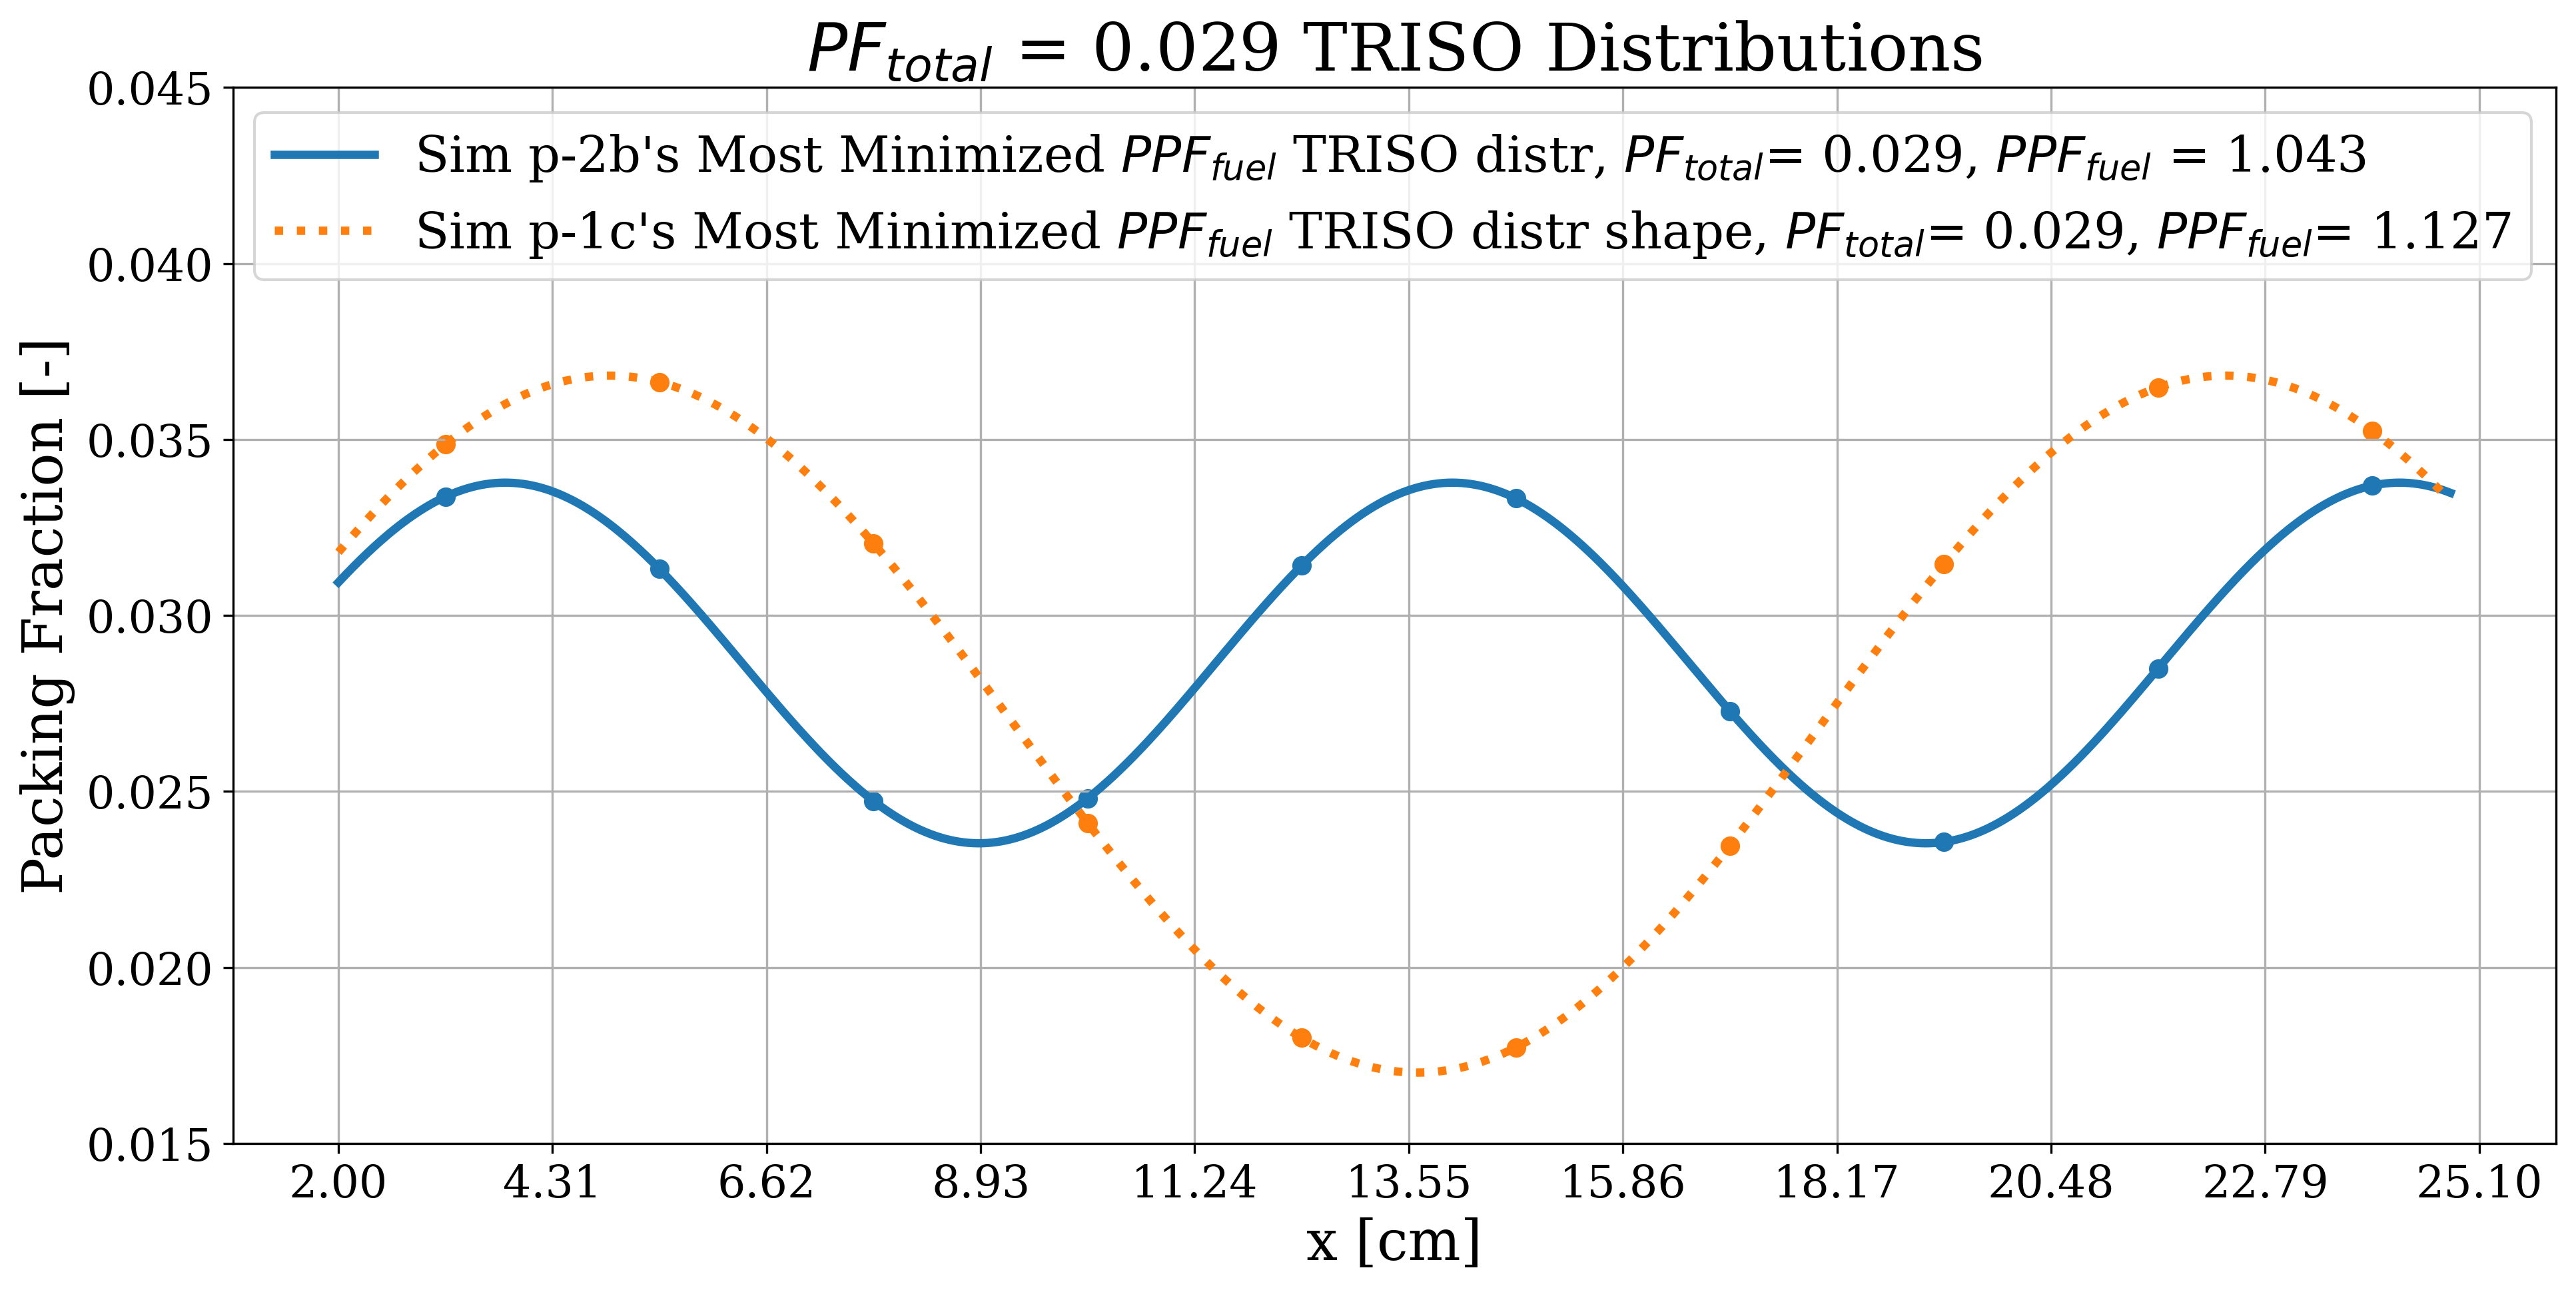
\includegraphics[width=0.9\linewidth]{triso-0.029.png} 
    \caption{Simulation p-2b's most-minimized $PPF_{fuel}$ TRISO distribution 
    from Figure \ref{fig:slab-obj-2-pfppf} and the constant $PF_{total}$ = 0.0292
    TRISO distribution.}
    \label{fig:triso-0.0292}
\end{figure}

Figure \ref{fig:flux-comparison-0.0292-plank} compares the flux distributions between 
simulation p-2b's most-minimized $PPF_{fuel}$ TRISO distribution and the
constant $PF_{total}$ = 0.0292 TRISO distribution (both shown in Figure 
\ref{fig:triso-0.0292}).
\begin{figure}[htbp!]
    \centering
    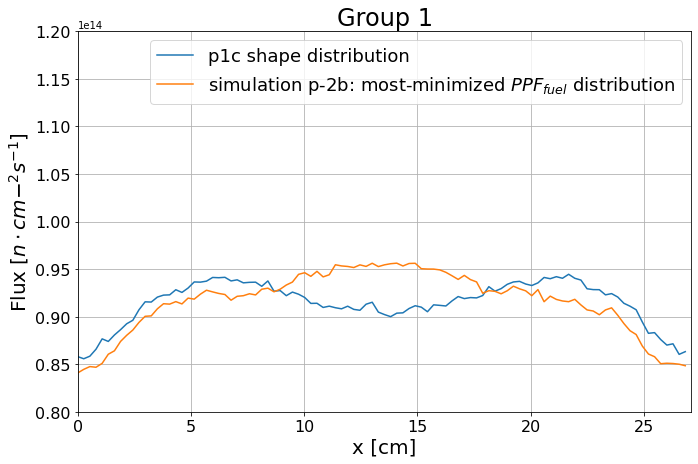
\includegraphics[width=0.48\linewidth]{flux-comparison-0.0292-plank_grp1.png} 
    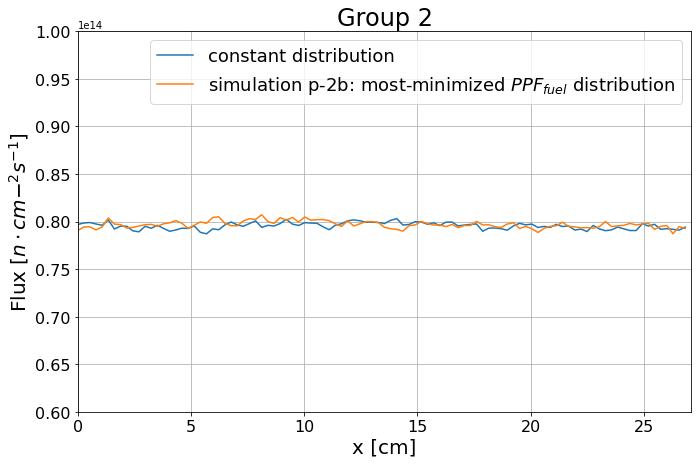
\includegraphics[width=0.48\linewidth]{flux-comparison-0.0292-plank_grp2.png} 
    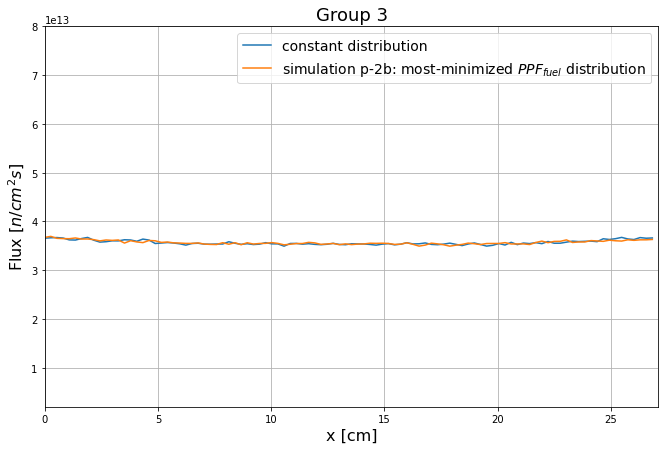
\includegraphics[width=0.48\linewidth]{flux-comparison-0.0292-plank_grp3.png} 
    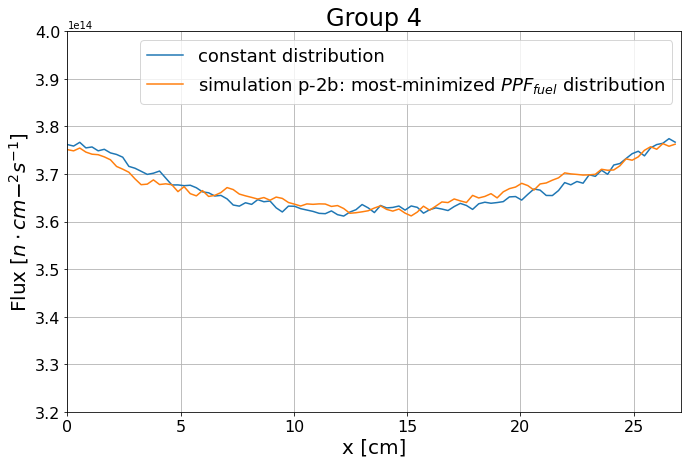
\includegraphics[width=0.48\linewidth]{flux-comparison-0.0292-plank_grp4.png} 
    \caption{Flux comparison between Figure \ref{fig:slab-obj-2-pfppf}'s TRISO 
    distribution that most-minimized $PPF_{fuel}$ and a constant $PF_{total}$ = 0.0292 
    TRISO distribution. 
    \acrfull{AHTR} plank's centerline neutron flux distribution in 4 groups at 948K. 
    Centerline is the white line in Figure \ref{fig:ahtr-plank-verification}.
    Energy Group 1: E $> 9.1188 \times 10^{-3}$ MeV, 
    Energy Group 2: $2.9023 \times 10^{-5} < E < 9.1188 \times 10^{-3}$ MeV,
    Energy Group 3:  $1.8556 \times 10^{-5} < E < 2.9023 \times 10^{-5}$ MeV,
    Energy Group 4:  $1.0 \times 10^{-12} < E < 1.8554 \times 10^{-6}$ MeV.}
    \label{fig:flux-comparison-0.0292-plank}
\end{figure}

Table \ref{tab:flux-comparison-0.0292-plank} quantifies the flux comparison 
from Figure \ref{fig:flux-comparison-0.0292-plank} between simulation p-2b's 
most-minimized $PPF_{fuel}$ TRISO distribution and the constant 
$PF_{total}$ = 0.0292 TRISO distribution (both shown in Figure \ref{fig:triso-0.0292}).
\begin{table}[htbp!]
    \centering
    \onehalfspacing
    \caption{Flux value comparison between Figure \ref{fig:slab-obj-2-pfppf}'s TRISO 
    distribution that most-minimized $PPF_{fuel}$ and a constant $PF_{total}$ = 0.0292 
    TRISO distribution. 
    Energy Group 1: E $> 9.1188 \times 10^{-3}$ MeV, 
    Energy Group 2: $2.9023 \times 10^{-5} < E < 9.1188 \times 10^{-3}$ MeV,
    Energy Group 3:  $1.8556 \times 10^{-5} < E < 2.9023 \times 10^{-5}$ MeV,
    Energy Group 4:  $1.0 \times 10^{-12} < E < 1.8554 \times 10^{-6}$ MeV.}
	\label{tab:flux-comparison-0.0292-plank}
    \footnotesize
    \begin{tabular}{lp{4cm}p{3.3cm}p{4cm}}
    \hline
    \textbf{Energy Group} &
    \textbf{$max(\phi)/min(\phi)$ most-minimized $PPF_{fuel}$ TRISO distribution} & 
    \textbf{$max(\phi)/min(\phi)$ constant TRISO distribution} & 
    \textbf{$\%$ difference (most minimized - constant)}\\
    \hline 
    1 & 1.137 & 1.152 & \Minus1.31 \\
    2 & 1.025 & 1.020 & \Plus0.49 \\
    3 & 1.057 & 1.051 & \Plus0.56 \\
    4 & 1.042 & 1.045 & \Minus0.28 \\
    \hline
    \end{tabular}
\end{table}

In energy group 4, the most-minimized $PPF_{fuel}$ TRISO distribution has 
$\sim 0.02$ TRISO variation and its flux distribution is $0.28\%$ flatter 
than the constant $PF_{total}$ = 0.0292 flux distribution, resulting in a lower 
$PPF_{fuel}$. 
In the previous section, simulation p-1c's most-minimized $PPF_{fuel}$ TRISO distribution 
has $\sim 0.07$ TRISO variation and its flux distribution is $3.96\%$ flatter than 
the constant $PF_{total}$ = 0.0979 flux distribution.  
Higher $PF_{total}$ in simulation p-1c means that there is more fuel, resulting in 
more self-shielding effects. 
This results in TRISO distribution variation having a stronger effect in neutralizing 
self-shielding. 

\paragraph{Simulation p-1f}
In Section \ref{sec:plank-1-obj-ppf}'s simulation p-1f, I conducted a single-objective 
optimization simulation to minimize fuel-normalized power peaking factor ($PPF_{fuel}$) 
by varying coolant channel shape.
Comparison of simulation p-1c and p-1f's results in Figures 
\ref{fig:slab-obj-1-ppf-evol-coolant} and \ref{fig:slab-obj-1-ppf-evol}
show that coolant channel shape variation barely has an impact on $PPF_{fuel}$ as 
\gls{TRISO} distribution variation: the average $PPF_{fuel}$ due to \gls{TRISO} 
variation decreased by 0.1 over 10 generations, while average $PPF_{fuel}$ due to 
coolant channel shape variation only decreased negligibly over 10 generations. 
Figure \ref{fig:slab-obj-1-ppf-final-coolant} reiterates that there is no correlation 
between total radius and $PPF_{fuel}$. 

\paragraph{Summary}
The minimize $PPF_{fuel}$ objective is driven by flattening thermal (Group 4) flux 
distribution. 
The minimize $PPF_{fuel}$ objective has correlations with the following input parameters: 
$PF_{total}$ and TRISO packing fraction distribution. 
The objective has no correlation with coolant channel shape input parameter.

\subsection{Discussion: Multi-Objective Optimization}
\label{sec:plank-discussion-multi}
\gls{ROLLO} successfully found widely spread solutions in each of the multi-objective 
optimization simulation's final generation Pareto fronts.
In this section, I explain how the driving factors and phenomena observed in 
the previous single-objective discussions (Sections 
\ref{sec:plank-discussion-pf}, \ref{sec:plank-discussion-temp}, and 
\ref{sec:plank-discussion-ppf}) combine to result in the optimal reactor models found 
by the multi-objective optimization simulations. 

\subsubsection{Simulation p-2a}
In Section \ref{sec:p-2a}'s simulation p-2a, I conducted two-objective 
optimization simulations to minimize total fuel packing fraction ($PF_{total}$) and 
maximum plank temperature ($T_{max}$) by varying TRISO distribution. 
\gls{ROLLO} found six widely spread reactor models on simulation p-2a's Pareto 
front (Figure \ref{fig:slab-obj-2-pftemp}). 

In simulation p-2a, \gls{ROLLO} found that the reactor model with the 
most-minimized $PF_{total}$ objective has an oscillating TRISO distribution with 
$\sim0.015$ variation and $PF_{total}=0.02$
(the blue distribution in Figure \ref{fig:slab-obj-2-pftemp-pareto-distr}). 
This distribution is similar to simulation p-1a's most-minimized $PF_{total}$ TRISO 
distribution (Figure \ref{fig:slab-obj-1-pf-final}), but differs as it varies between 
0.005 and 0.035, instead of 0 and 0.4, due to influences from the minimize $T_{max}$ 
objective. 
In simulation p-2a, \gls{ROLLO} found that the reactor model with the most-minimized 
$T_{max}$ objective has a constant TRISO distribution with $PF_{total} = 0.032$
(the purple distribution in Figure \ref{fig:slab-obj-2-pftemp-pareto-distr}).
This distribution follows a similar flat shape as simulation p-1b's most-minimized 
$T_{max}$ TRISO distribution (Figure \ref{fig:slab-obj-1-temp-final}).

The \gls{TRISO} distributions on the Pareto front in Figure \ref{fig:slab-obj-2-pftemp} 
minimize both $PF_{total}$ and $T_{max}$, they vary between the two extreme cases: 
most-minimized $PF_{total}$ and most-minimized $T_{max}$. 
The minimize $T_{max}$ objective influences the TRISO distribution's flatness as 
described in Section \ref{sec:plank-discussion-temp}, while 
the minimize $PF_{total}$ objective influences the oscillating pattern, as described 
in Section \ref{sec:plank-discussion-pf}.

\subsubsection{Simulation p-2b}
In Section \ref{sec:p-2b}'s simulation p-2b, I conducted a two-objective 
optimization simulation to minimize total fuel packing fraction ($PF_{total}$) and 
fuel-normalized power peaking factor ($PPF_{fuel}$) by varying TRISO distribution. 
\gls{ROLLO} found four widely spread reactor models on simulation p-2b's Pareto 
front. 

In simulation p-2b, \gls{ROLLO} found that the reactor model with the most-minimized 
$PF_{total}$ objective has a constant TRISO distribution and $PF_{total} = 0.02$
(the orange distribution in Figure \ref{fig:slab-obj-2-pfppf-pareto-distr}). 
This distribution differs from simulation p-1a's most-minimized $PF_{total}$ oscillating 
TRISO distribution. 
Table \ref{tab:0.023-plank-ppf} reports the $PPF_{fuel}$ values for simulation p-1a's 
most-minimized $PF_{total}$ ($PF_{total} = 0.023$) oscillating TRISO distribution and 
a constant $PF_{total} = 0.023$ TRISO distribution (both distributions shown 
in Figure \ref{fig:triso-0.023}).
\begin{table}[htbp!]
    \centering
    \onehalfspacing
    \caption{Fuel-normalized power peaking factor ($PPF_{fuel}$) comparison between  
    simulation p-1a's most-minimized $PF_{total}$ TRISO distribution and a 
    constant $PF_{total}$ = 0.023 TRISO distribution.}
	\label{tab:0.023-plank-ppf}
    \footnotesize
    \begin{tabular}{ll}
    \hline
    \textbf{TRISO distribution} & \textbf{$PPF_{fuel}$ [-]} \\
    \hline 
    Most-minimized $PF_{total}$ & 1.363 \\
    Constant $PF_{total}$ = 0.023 & 1.063 \\
    \hline
    \end{tabular}
\end{table}

Table \ref{tab:0.023-plank-ppf} shows that simulation p-1a's most-minimized $PF_{total}$ 
oscillating TRISO distribution has a large $PPF_{fuel} = 1.363$.
The influences from the minimize $PPF_{fuel}$ objective explains why for simulation p-2b, 
\gls{ROLLO} found that the reactor model that most-minimized $PF_{total}$ has a 
constant TRISO distribution instead of an oscillating TRISO distribution.

In simulation p-2b, \gls{ROLLO} found that the reactor model with the most-minimized 
$PPF_{fuel}$ has a TRISO distribution that peaks in the plank's center and both sides 
with a $\sim0.02$ variation and $PF_{total}=0.029$ (the blue distribution in Figure 
\ref{fig:slab-obj-2-pfppf-pareto-distr}). 
This distribution differs from simulation p-1c's most-minimized $PPF_{fuel}$ TRISO 
distribution (Figure \ref{fig:slab-obj-1-ppf-final}) which has a large $\sim 0.07$ 
variation in TRISO distribution with a minimum point in the center of the plank. 
Section \ref{sec:plank-discussion-ppf-results} discussed the reasoning for the 
difference between the most-minimized $PPF_{fuel}$ TRISO distributions in 
simulation p-2b and p-1c. 

Unlike simulations p-2a and p-2c, simulation p-2b's extreme most-minimized $PF_{total}$ 
and most-minimized $PPF_{fuel}$ do not follow similar results as their single-objective 
counterparts.  
The results from simulation p-2b and investigations in Section 
\ref{sec:plank-discussion-ppf-results} suggest that the minimize $PF_{total}$ 
objective's driving factor maximize total fission reaction rate and 
minimize $PPF_{fuel}$ objective's driving factor flattening thermal flux distribution 
influence each other resulting in unexpected TRISO distributions based 
on the value of $PF_{total}$. 

\subsubsection{Simulation p-2c}
In Section \ref{sec:p-2c}'s simulation p-2c, I conducted a two-objective 
optimization simulation to minimize maximum plank temperature ($T_{max}$) and 
fuel-normalized power peaking factor ($PPF_{fuel}$) by varying TRISO distribution. 
\gls{ROLLO} found eight widely spread reactor models on simulation p-2c's Pareto 
front. 

In simulation p-2c, \gls{ROLLO} found that the reactor model with the most-minimized 
$T_{max}$ has a slightly oscillating TRISO distribution
(the orange distribution in Figure \ref{fig:slab-obj-2-tempppf-pareto-distr}). 
This distribution follows a similar flat shape as simulation p-1b's most-minimized 
$T_{max}$ TRISO distribution (Figure \ref{fig:slab-obj-1-temp-distr}).
In simulation p-2c, \gls{ROLLO} found that the reactor model with the most-minimized 
$PPF_{fuel}$ has a TRISO distribution with peaks near the sides of the plank and a 
minimum point at the plank's center (the grey distribution in Figure 
\ref{fig:slab-obj-2-tempppf-pareto-distr}). 
This distribution is somewhat similar to p-1c's most-minimized $PPF_{fuel}$ TRISO 
distribution (Figure \ref{fig:slab-obj-1-ppf-final}) which also has a minimum point 
at the center of the plank, but differs as its peaks are on the fuel regions' edges 
instead of the plank's edges. 

The \gls{TRISO} distributions on the Pareto front in Figure \ref{fig:slab-obj-2-tempppf} 
minimize both $T_{max}$ and $PPF_{fuel}$, they vary between the two extreme cases: 
most-minimized $T_{max}$ and most-minimized $PPF_{fuel}$. 
The minimize $T_{max}$ objective influences the TRISO distribution's flatness as 
described in Section \ref{sec:plank-discussion-temp}.
Simulation p-2c holds $PF_{total}$ constant at 0.0979. 
The minimize $PPF_{fuel}$ objective influences the TRISO distribution to follow 
a similar shape to simulation p-1c (also $PF_{total} = 0.0979$) with a minimum point in 
plank's center and a TRISO variation of $\sim0.07$ to flatten thermal flux, as 
described in Section \ref{sec:plank-discussion-ppf}. 

\subsubsection{Simulation p-3a}
In Section \ref{sec:p-3a}'s simulation p-3a, I conducted a three-objective 
optimization simulation to minimize total fuel packing fraction ($PF_{total}$), 
maximum plank temperature ($T_{max}$), and fuel-normalized power peaking factor 
($PPF_{fuel}$) by varying $PF_{total}$ and TRISO distribution.
\gls{ROLLO} found 14 widely spread reactor models on simulation p-3a's Pareto 
front. 

In simulation p-3a, \gls{ROLLO} found that the reactor model with the most-minimized 
$T_{max}$ has a flat TRISO distribution and $PF_{total} = 0.059$
(the orange distribution in Figure \ref{fig:slab-obj-3-distr-most-minimized}). 
This distribution follows a similar flat shape as simulation p-1b's most-minimized 
$T_{max}$ TRISO distribution (Figure \ref{fig:slab-obj-1-temp-distr}).
In simulation p-3a, \gls{ROLLO} found that the reactor model with the most-minimized 
$PF_{total}$ has an oscillating TRISO distribution and $PF_{total} = 0.02$
(the purple distribution in Figure \ref{fig:slab-obj-3-distr-most-minimized}). 
This distribution is similar to simulation p-1a's most-minimized $PF_{total}$ TRISO 
distribution (Figure \ref{fig:slab-obj-1-pf-final}) with an oscillating TRISO 
distribution.
In simulation p-3a, \gls{ROLLO} found that the reactor model with the most-minimized 
$PPF_{fuel}$ has a slightly oscillating TRISO distribution and $PF_{total} = 0.025$ 
(the pink distribution in Figure \ref{fig:slab-obj-3-distr-most-minimized}). 

Most of the \gls{TRISO} distributions on the Pareto front (Figure 
\ref{fig:slab-obj-3-distr}) have a mostly flat distribution with approximately 
$\sim0.01cm$ of variation. 
The flatness is influenced by the minimize $T_{max}$ objective. 
The variations in \gls{TRISO} distributions are influenced by both the minimize 
total packing fraction and minimize $PPF_{fuel}$ objectives. 
However, as mentioned previously, the $PF_{total}$ and $PPF_{fuel}$ relationship
results in unexpected TRISO distributions at different $PF_{total}$ values. 
The minimize $PF_{total}$ objective tries to maximize fission reaction rate
to enable a higher $k_{eff}$ for lower $PF_{total}$, and 
the $PPF_{fuel}$ objective tries to flatten thermal flux. 

\subsubsection{Simulation p-3b}
In Section \ref{sec:p-3b}'s simulation p-3b, I conducted a three-objective 
optimization simulation to minimize total fuel packing fraction ($PF_{total}$), 
maximum plank temperature ($T_{max}$), and fuel-normalized power peaking factor 
($PPF_{fuel}$) by varying $PF_{total}$, TRISO distribution, and coolant channel shape.
\gls{ROLLO} found 21 widely spread reactor models on simulation p-3b's Pareto 
front. 

In simulation p-3b, \gls{ROLLO} found that the reactor model with the most-minimized 
$T_{max}$ has a constant TRISO distribution, $PF_{total} = 0.034$, and $r_{tot}=0.657cm$ 
(the dark green distribution in Figure 
\ref{fig:slab-obj-3-distr-most-minimized-distr-all}).
This distribution follows a similar flat shape as simulation p-1b's most-minimized 
$T_{max}$ TRISO distribution (Figure \ref{fig:slab-obj-1-temp-distr}) and has a large 
$r_{top}$ and $r_{bot}$ due to the negative correlation between $T_{max}$ and $r_{tot}$
found in simulation p-1e (Sections \ref{sec:plank-1-obj-temp} and 
\ref{sec:plank-discussion-temp}). 

In simulation p-3b, \gls{ROLLO} found that the reactor model with the most-minimized 
$PF_{total}$ has an oscillating TRISO distribution with $\sim0.01$ variation, 
$PF_{total} = 0.026$, and $r_{tot}=0.505cm$
(the pink distribution in Figure \ref{fig:slab-obj-3-distr-most-minimized-distr-all}).
This distribution is similar to simulation p-1a's most-minimized $PF_{total}$ TRISO 
distribution (Figure \ref{fig:slab-obj-1-pf-final}) with an oscillating TRISO 
distribution.
Simulation p-1d concluded that there was no correlation between $PF_{total}$ and $r_{tot}$, 
thus, the large $r_{tot}$ value is only influenced by the minimize $T_{max}$ objective. 

In simulation p-3b, \gls{ROLLO} found that a TRISO distribution that has a 
constant TRISO distribution, $PF_{total} = 0.036$, and $r_{tot}=0.307cm$ most-minimized 
$PPF_{fuel}$ (the light green distribution in Figure 
\ref{fig:slab-obj-3-distr-most-minimized-distr-all}).
The constant TRISO distribution is unexpected for the most-minimized $PPF_{fuel}$ result. 
However, as mentioned before the $PF_{total}$ and $PPF_{fuel}$ relationship
results in unexpected TRISO distributions at different $PF_{total}$ values. 

Similar to simulation p-3a, most of the \gls{TRISO} distributions on simulation 
p-3b's Pareto front (Figure \ref{fig:slab-obj-3-distr-all}) have a mostly flat 
distribution with approximately $\sim0.01cm$ of variation. 
Most of the Pareto front's $r_{tot}$ are large due to the minimize $T_{max}$ objective. 
The TRISO distribution's flatness is influenced by the minimize $T_{max}$ objective. 
The variations in \gls{TRISO} distributions are influenced by both the minimize 
total packing fraction and minimize $PPF_{fuel}$ objectives. 
However, as mentioned previously, the $PF_{total}$ and $PPF_{fuel}$ relationship
results in unexpected TRISO distributions at different $PF_{total}$ values. 
The minimize $PF_{total}$ objective tries to maximize fission reaction rate
to enable a higher $k_{eff}$ for lower $PF_{total}$, and 
the $PPF_{fuel}$ objective tries to flatten thermal flux. 

\subsection{Discussion: Major Takeaways}
In Section \ref{sec:plank-discussion}, I conducted investigations to understand the 
driving factors for each individual objective, and how their combined effects 
result in the optimal reactor models found by the multi-objective optimization 
simulations. 

The minimize $T_{max}$ objective is driven by minimizing plank's maximum temperature; 
and flattens TRISO distribution and maximizes coolant channel shape's $r_{tot}$ to 
achieve the objective. 
The minimize $PF_{total}$ objective is driven by maximizing the plank's total fission 
reaction rate and influences the TRISO disribution to achieve the objective. 
The minimize $PPF_{fuel}$ objective is driven by flattening the plank's thermal flux
distribution and influences $PF_{total}$ and TRISO disribution to achieve the objective. 
Both the minimize $PF_{total}$ and minimize $PPF_{fuel}$ objectives have no correlation 
with the coolant channel shape. 
The results from simulation p-2b and investigations in Section 
\ref{sec:plank-discussion-ppf-results} suggest that the minimize $PF_{total}$ 
objective's driving factor maximize total fission reaction rate and 
minimize $PPF_{fuel}$ objective's driving factor flattening thermal flux distribution 
influence each other resulting in unexpected TRISO distributions based 
on the value of $PF_{total}$. 

All these effects and influences come together in each multi-objective optimization 
simulation to give a set of optimal reactor models on a Pareto front. 
Simulation p-3b's multi-objective optimization shows the result of minimizing all 
three objectives (minimize $PF_{total}$, $T_{max}$, and $PPF_{fuel}$) while varying 
all the input parameters ($PF_{total}$, TRISO distribution, and coolant channel shape).
Figure \ref{fig:slab-obj-3-all} shows the 21 widely spread reactor models on simulation 
p-3b's Pareto front. 

\pagebreak
\section{Summary}
\glsresetall
This chapter described the \gls{AHTR} plank's \gls{ROLLO} optimization results. 
I varied the following \gls{AHTR} plank input parameters: \gls{TRISO} packing fraction 
distribution ($\rho_{TRISO}(\vec{r})$), total fuel packing fraction ($PF_{total}$), and 
coolant channel shape; in an effort to minimize the following objectives: total 
fuel packing fraction ($PF_{total}$), maximum plank temperature ($T_{max}$), and 
fuel-normalized power peaking factor ($PPF_{fuel}$). 

In Section \ref{sec:plank-one-obj}'s six single-objective optimization simulations: 
p-1a, p-1b, p-1c, p-1d, p-1e, p-1f; and Sections \ref{sec:plank-discussion-pf}, 
\ref{sec:plank-discussion-temp}, and \ref{sec:plank-discussion-ppf} discussions    
I characterized each objective's driving factors and relationship with each input 
parameter. 
I determined that the minimize $T_{max}$ objective is driven by minimizing plank's maximum 
temperature; and flattens TRISO distribution and maximizes coolant channel shape's 
$r_{tot}$ to achieve the objective. 
The minimize $PF_{total}$ objective is driven by maximizing the plank's total fission 
reaction rate and influences the TRISO disribution to achieve the objective. 
The minimize $PPF_{fuel}$ objective is driven by flattening the plank's thermal flux
distribution and influences $PF_{total}$ and TRISO disribution to achieve the objective. 
Both the minimize $PF_{total}$ and minimize $PPF_{fuel}$ objectives have no correlation 
with the coolant channel shape. 

In Sections \ref{sec:plank-two-obj} and \ref{sec:plank-three-obj}'s five multi-objective 
optimization simulations: p-2a, p-2b, p-2c, p-3a, and p-3b; and Section 
\ref{sec:plank-discussion-multi}'s discussions, I further analyzed how the objectives' 
combined effects resulted in the optimal reactor models found by each multi-objective 
optimization simulation. 
All the multi-objective optimization simulations successfully found a wide spread of 
reactor models on a Pareto front that meets each objective to varying degrees. 
In the multi-objective optimization simulations, the minimize $T_{max}$ objective 
continued to influence the flattening of the TRISO distribution and maximizing of the 
coolant channel shape's $r_{tot}$ to achieve the objective. 
The results from simulation p-2b and investigations in Section 
\ref{sec:plank-discussion-ppf-results} suggested that the minimize $PF_{total}$ 
objective's driving factor maximize total fission reaction rate and 
minimize $PPF_{fuel}$ objective's driving factor flattening thermal flux distribution 
influence each other resulting in unexpected TRISO distributions based 
on the value of $PF_{total}$. 
Simulation p-3b's multi-objective optimization shows the result of minimizing all 
three objectives (minimize $PF_{total}$, $T_{max}$, and $PPF_{fuel}$) while varying 
all the input parameters ($PF_{total}$, TRISO distribution, and coolant channel shape).
Figure \ref{fig:slab-obj-3-all} shows the 21 widely spread reactor models on simulation 
p-3b's Pareto front that meet the three objectives to varying degrees. 

This chapter demonstrated \gls{ROLLO}'s success in conducting multi-objective 
optimization, a global search of the large reactor design space, to find optimal reactor 
models on the Pareto front that satisfy all the objectives. 
Reactor designers can utilize \gls{ROLLO} for multi-objective optimization problems with 
any number of objectives and arbitrary input parameters, to narrow down the search space 
to find reactor models that meet their desired requirements. 
The results from the multi-objective optimizations help reactor designers gain a clearer 
understanding of the reactor models' parameters that meet their defined objectives to 
varying degrees.
From there, reactor designers can determine the importance of each objective for 
their purposes, then conduct sensitivity analysis and use higher fidelity models to 
further study a smaller section of the optimal design space that they are 
interested in.

This chapter successfully determined and explained the driving factors behind 
each objective and their relationship with one another.  
Characterizations of each objective on a simple \gls{AHTR} plank model provides 
insights for the next chapter in which I conduct multi-objective optimization for 
the more complex \gls{AHTR} one-third assembly model. 
